%%%%%%%%%%%%%%%%%%%%%%%%%%%%%%%%%%%%%%%%%%%%%%%%%%%
%
%  New template code for TAMU Theses and Dissertations starting Fall 2016.
%
%
%  Author: Sean Zachary Roberson 
%	 Version 3.16.09
%  Last updated 9/12/2016
%
%%%%%%%%%%%%%%%%%%%%%%%%%%%%%%%%%%%%%%%%%%%%%%%%%%%

%%%%%%%%%%%%%%%%%%%%%%%%%%%%%%%%%%%%%%%%%%%%%%%%%%%%%%%%%%%%%%%%%%%%%%
%%                           APPENDIX A 
%%%%%%%%%%%%%%%%%%%%%%%%%%%%%%%%%%%%%%%%%%%%%%%%%%%%%%%%%%%%%%%%%%%%%

\phantomsection

\chapter{\uppercase{Full Results for In Band Testing}}\label{appendix_a}

The results of all 5 altimeters presented to the FSMP in~\cite{uwe_radio_2019} are presented here. The results were summarized in Table~\ref{tab:ib_thresholds_fsmp}. The breaking point was as described in Section~\ref{sub:break}, and consists of any reported altitude a) labeled NCD b) with a maximum height error $\geq\pm2\%$, or c) any mean height error $\geq\pm5\%$. Interference power thresholds were then set 2 dB below the breaking point of the worst performing altimeter (RA Type 4). 
 \begin{figure}[h!]
	\centering
	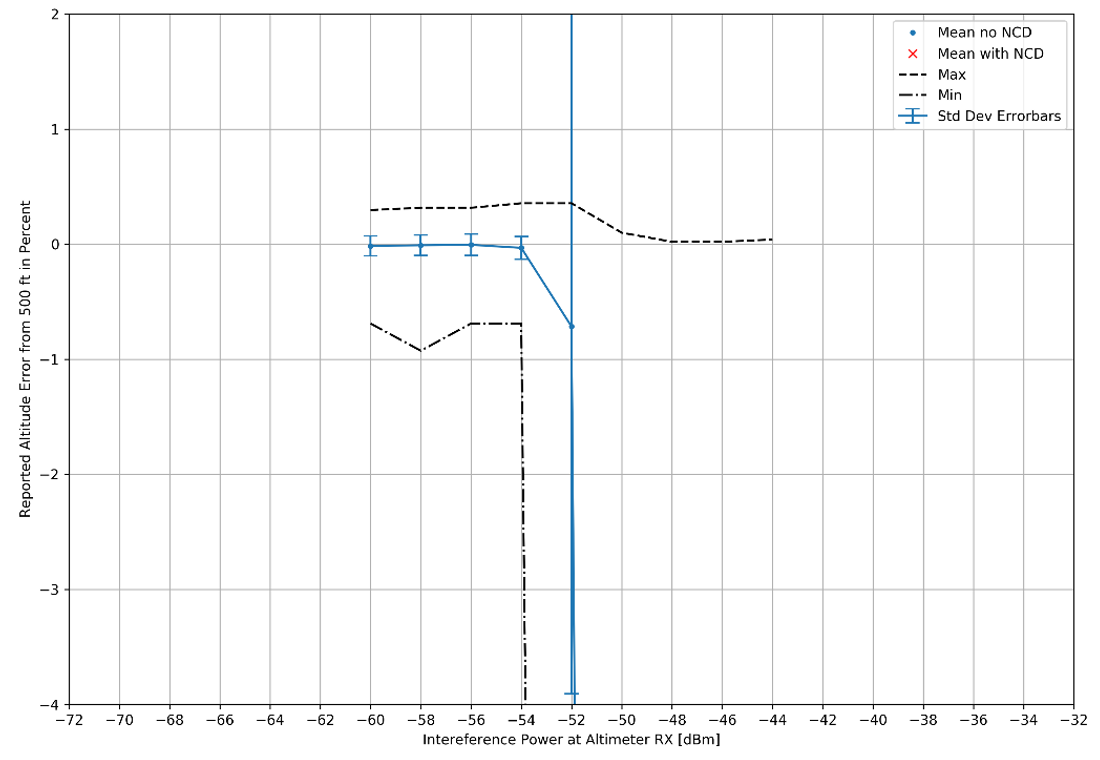
\includegraphics[width=5.0in]{RA1_ib_results.png}
	\caption{Performance of RA Type 1 with 200MHz In Band Tests}
	\label{fig:RA1}
\end{figure}

 \begin{figure}[h!]
	\centering
	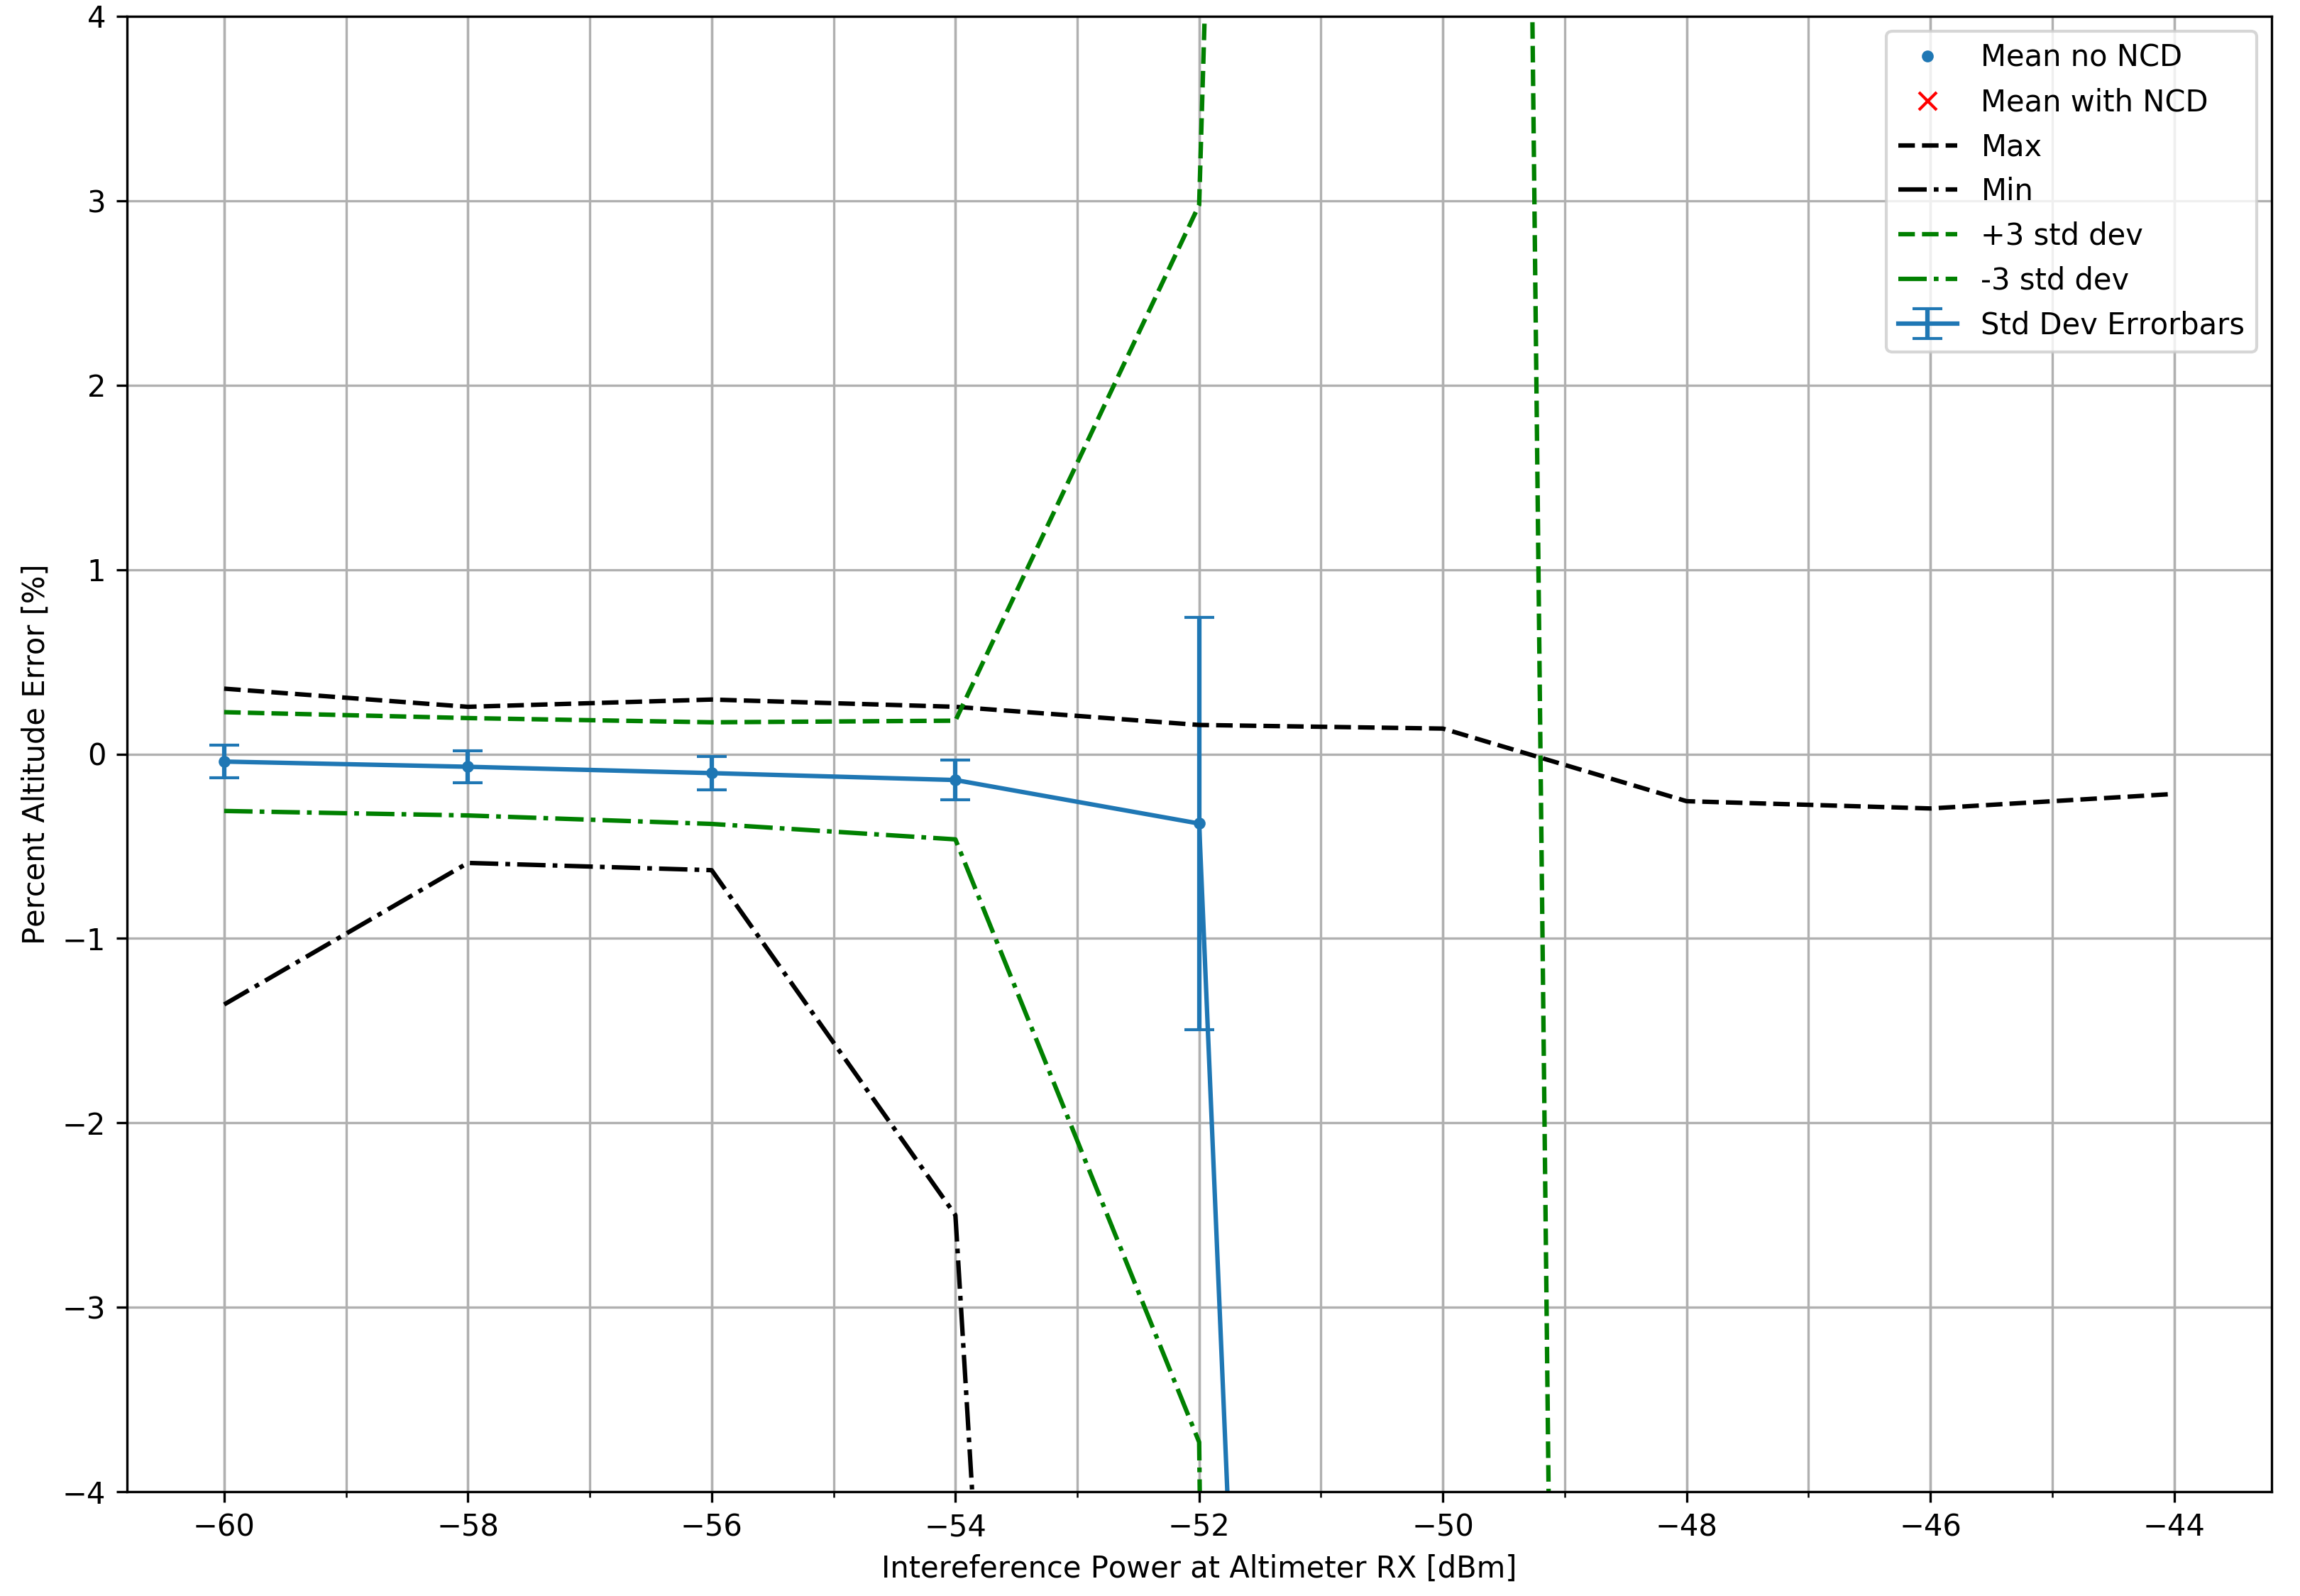
\includegraphics[width=5.0in]{RA2_ib_results.png}
	\caption{Performance of RA Type 2 with 200MHz In Band Tests}
	\label{fig:RA2}
\end{figure}

 \begin{figure}[h!]
	\centering
	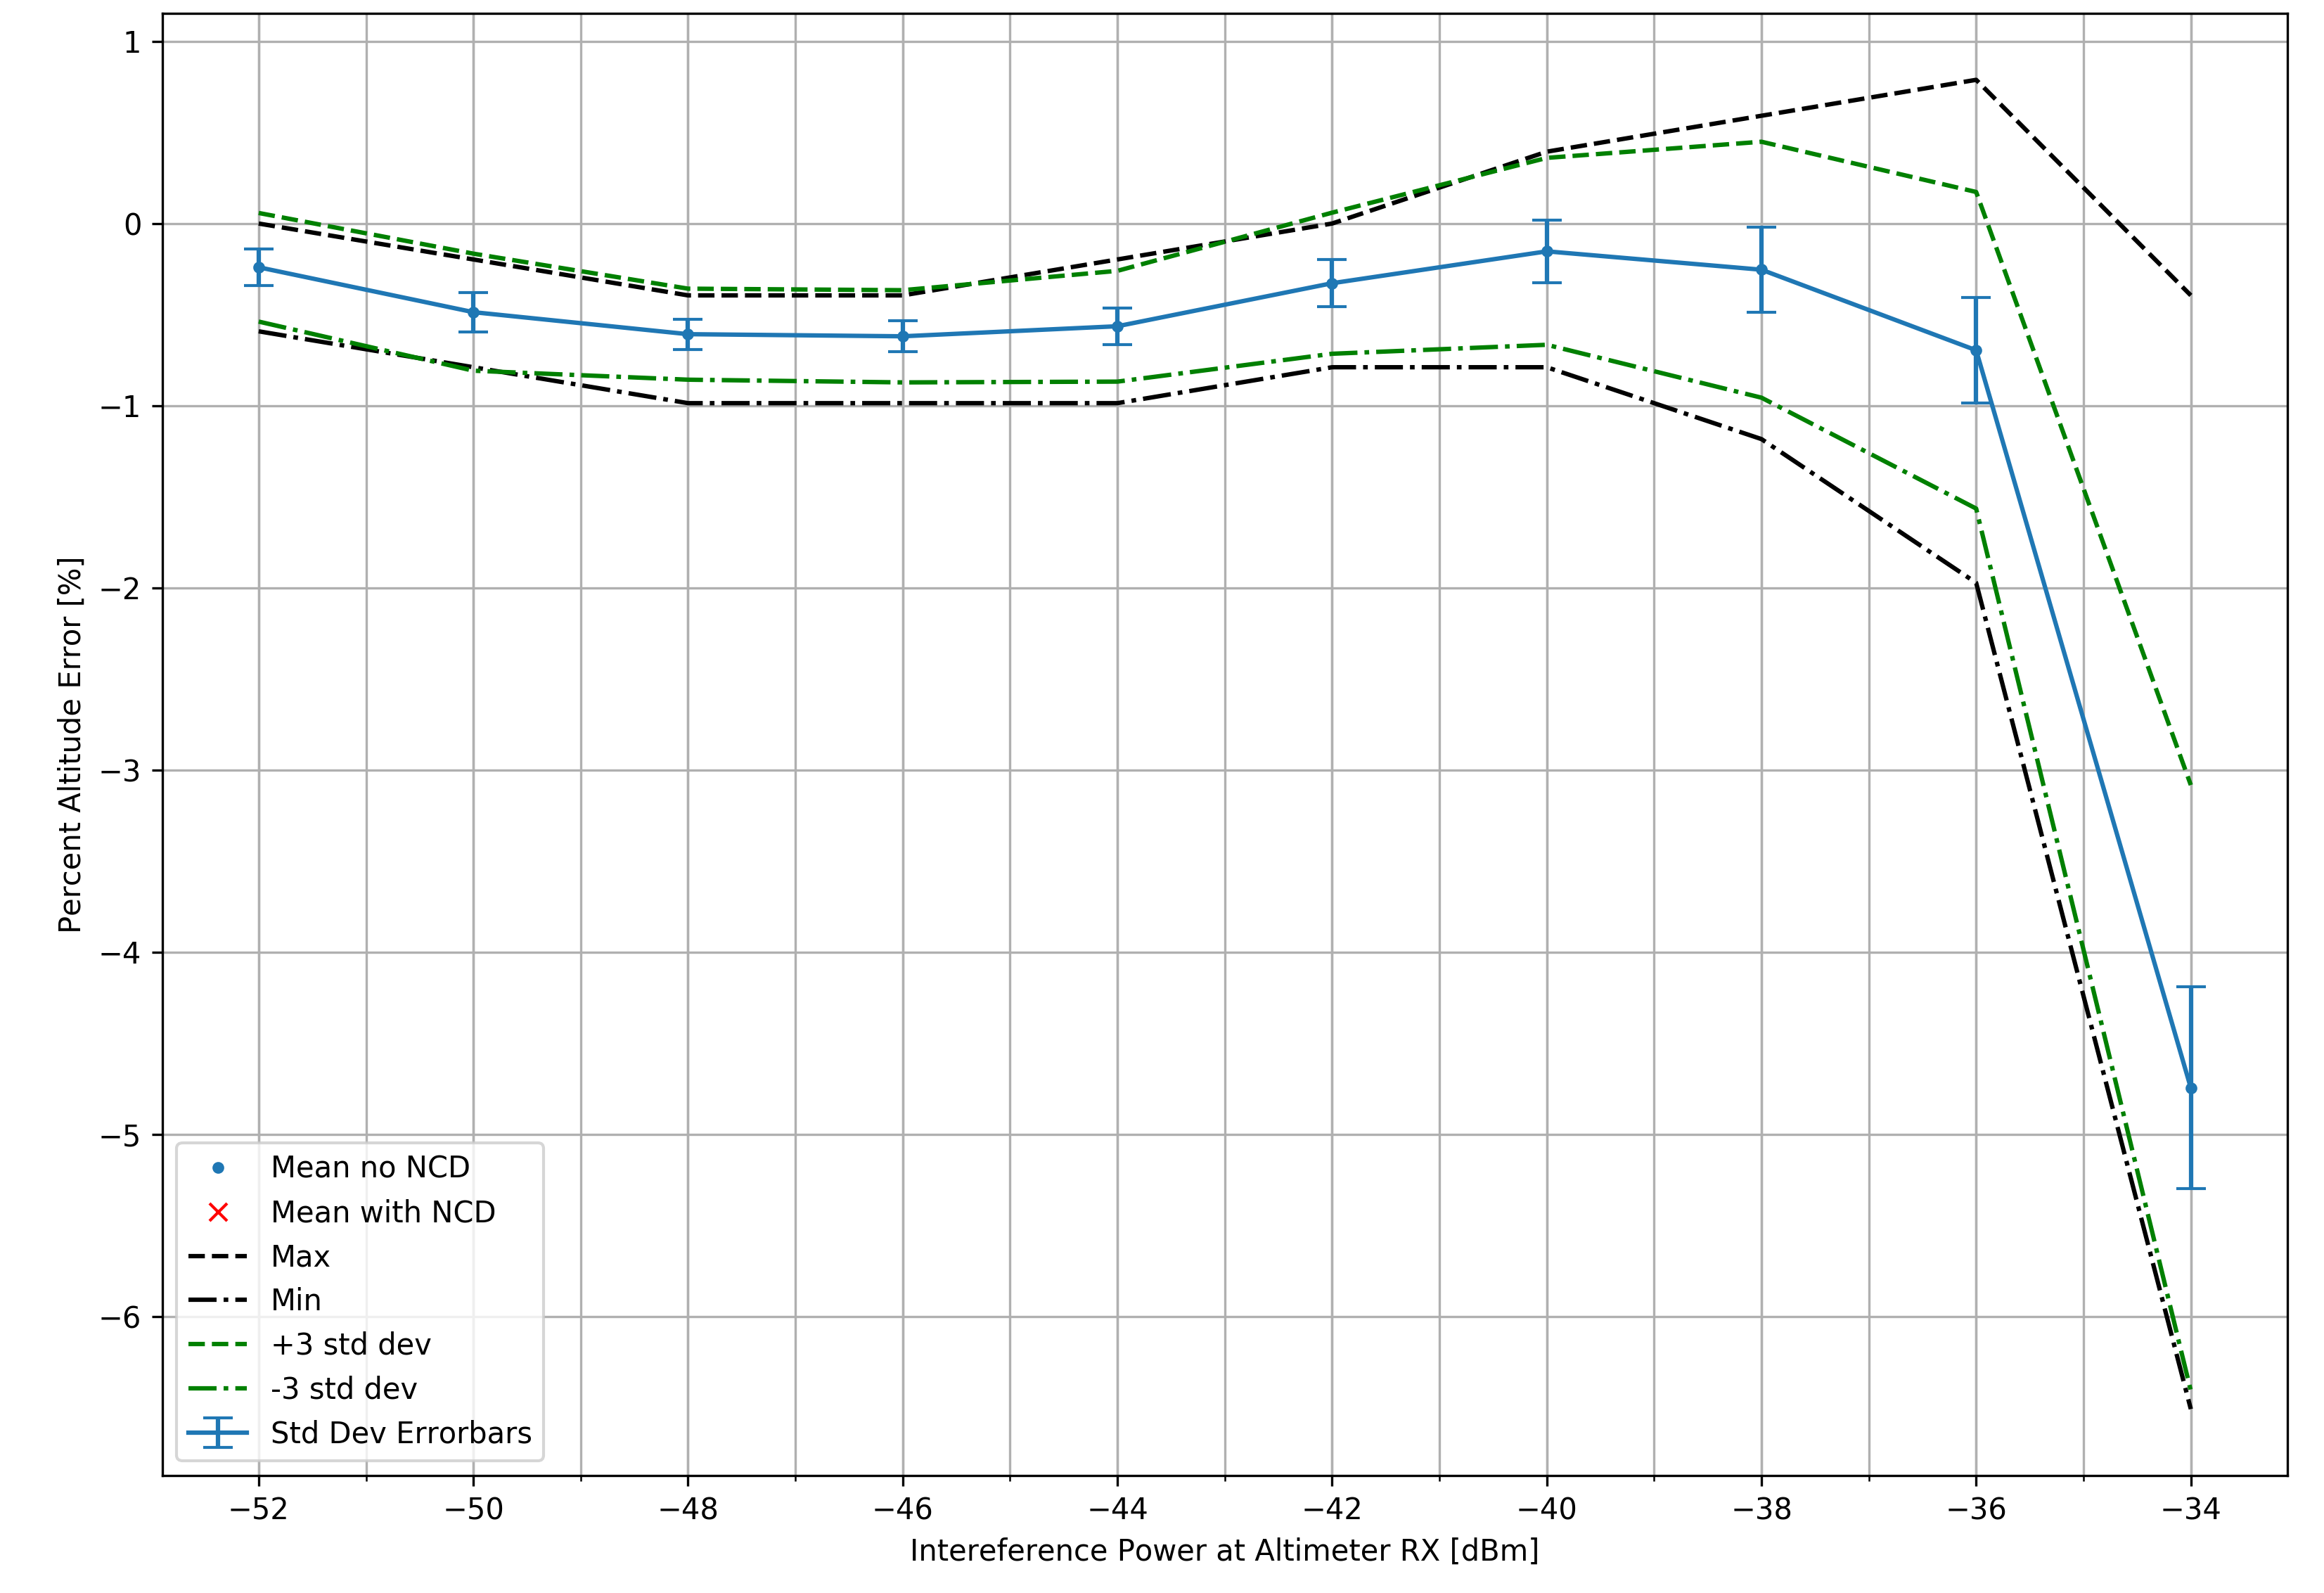
\includegraphics[width=5.0in]{RA3_ib_results.png}
	\caption{Performance of RA Type 3 with 200MHz In Band Tests}
	\label{fig:RA3}
\end{figure}

 \begin{figure}[h!]
	\centering
	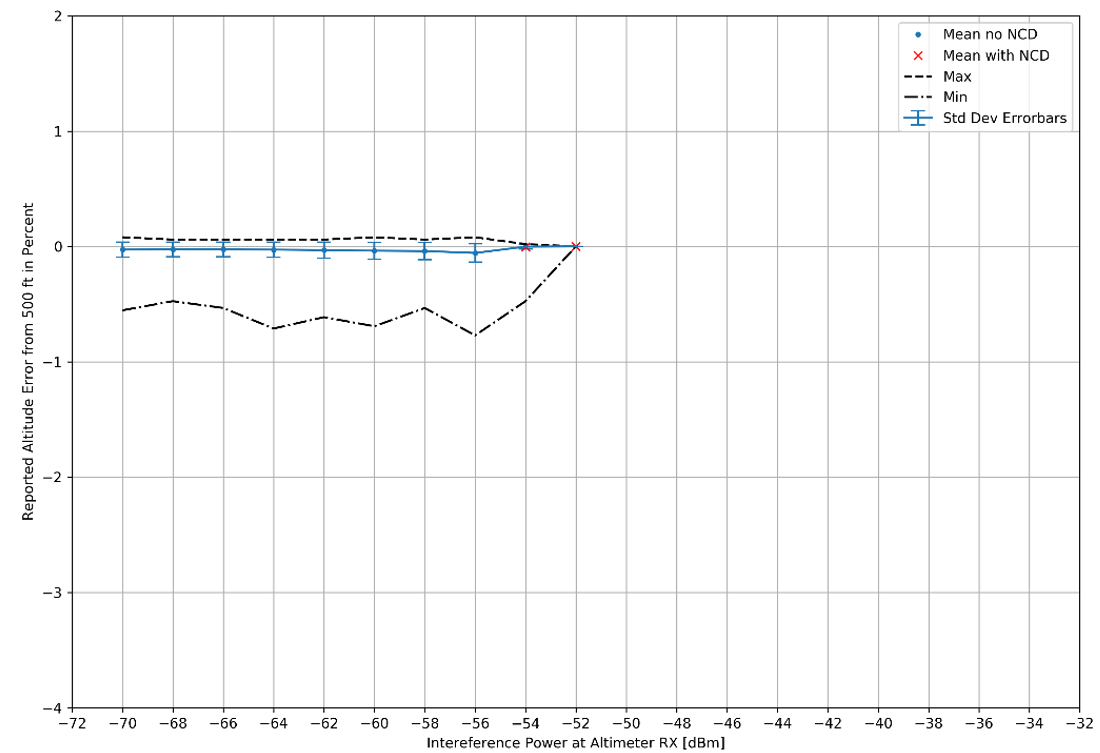
\includegraphics[width=5.0in]{RA4_ib_results.png}
	\caption{Performance of RA Type 4 with 200MHz In Band Tests}
	\label{fig:RA4_appendix}
\end{figure}

 \begin{figure}[h!]
	\centering
	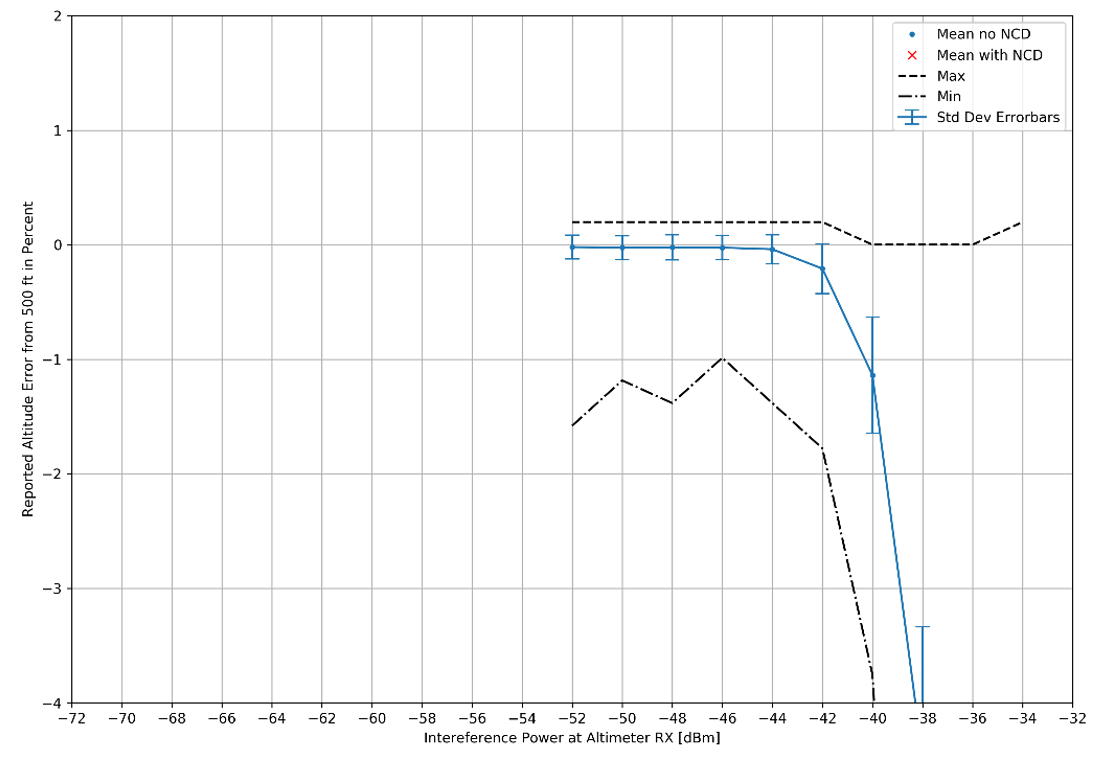
\includegraphics[width=5.0in]{RA5_ib_results.png}
	\caption{Performance of RA Type 5 with 200MHz In Band Tests}
	\label{fig:RA5}
\end{figure}
